%-------------------------------------------------------------------------
% Section: 前情提要
%-------------------------------------------------------------------------
\chapter{Preliminaries}
\label{cha:Preliminaries}
In this chapter, we introduce the background technology for our work. 
Embedded Linux, UIO Driver, AXI Bus, and DMA.


%-------------------------------------------------------------------------
% Section: 嵌入式理你斯
%-------------------------------------------------------------------------

\section{Embedded Linux}
\label{sec:Embedded Linux}

Embedded Linux is a kernel and set of libraries and utilitied designed to run
on an embedded system(for example:router). 

\subsection{Device Tree}
\label{subsec:Device Tree}

Device Tree is a mechanism to describe all hardware and devices of a system. In early Linux 
kernel, hardware description is hardcode in kernel file, so porting kernel to different
ARM-CPU based system is painful. To solve this problem, Device Tree is introduced. 
Like x86 based system, we should consider Linux kernel image is a black box, and give the 
hardware informations of system to kernel. \\
%
In FPGA development flow, the whole system keeps almost the same, the =only thing changes 
is our design in PL(Programmable Logic) side. To boot Linux with different PL design, only 
a little modification of devicetree file is needed.     


\subsection{Linux Kernel Driver}
\label{subsec:Linux Kernel Driver} 


%-------------------------------------------------------------------------
% Section: UIO driver
%-------------------------------------------------------------------------

\section{UIO}
\label{sec:UIO}
For many types of devices, creating a Linux kernel driver is overkill. All that is really needed 
is some way to handle an interrupt and provide access to the memory space of the device. To address 
this situation, the userspace I/O system (UIO) was designed.Hardware that is ideally suited for an 
UIO driver fulfills all of the following:
%
\begin{itemize}
\item The device has memory that can be mapped.
\item The device can be controlled completely by writing to this memory.
\item The device usually generates interrupts.
\item The device does not fit into one of the standard kernel subsystems.
\end{itemize}
%
Figure~\ref{fig:UIO Driver} shows how the UIO system works, in software-side of FPGA development, we 
only care about the value in the hardware register and when we can get the correct value, so memeory
-mapping to user-spcae application and interrupt handler is realy enough in our design flow.  
%
\begin{figure}[!htb]
  \centering
  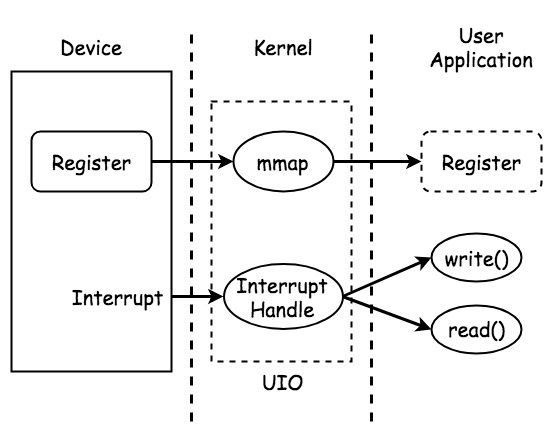
\includegraphics[scale=0.5]{images/uio.jpg}
  \caption[The UIO way.]{The UIO way.}
  \label{fig:UIO Driver}
\end{figure}

%-------------------------------------------------------------------------
% Section: AXI Bus
%-------------------------------------------------------------------------
\section{AXI Bus}
\label{sec:AXI Bus}

Advanced eXtensible Interface (AXI) protocol is part of ARM AMBA(Advanced Microcontroller Bus Architecture).
It is a on-chip bus interface that is targeted at high performance, high clock frequency system designs and includes features that make it suitable for high speed sub-micrometer interconnect:
\begin{itemize}
\item separate address/control and data phases
\item support for unaligned data transfers using byte strobes
\item burst based transactions with only start address issued
\item issuing of multiple outstanding addresses with out of order responses
\item easy addition of register stages to provide timing closure.
\end{itemize}

\subsection{AMBA}
\label{subsec:AMBA}


\subsection{AXI4}
\label{subsec:AXI4}
AXI4
\begin{itemize}
\item AXI4:
\item AXI4-Lite:
\item AXI4-Stream:
\end{itemize}





%-------------------------------------------------------------------------
% Section: DMA
%-------------------------------------------------------------------------
\section{DMA}
\label{sec:DMA}

\subsection{DMA Engine }
\label{subsec:DMA Engine}